\documentclass[fleqn]{article}
\usepackage[spanish]{babel}
\usepackage{amsmath}
\usepackage{amsthm}
\usepackage{graphicx}
\usepackage[utf8]{inputenc}

%%%%%%%% MARGIN
\usepackage[left=1in, right=1in, top=0.8in, bottom=0.8in]{geometry}

%%%%%%%% NO PARAGRAPH INDENT
% https://tex.stackexchange.com/questions/27802/set-noindent-for-entire-file
\setlength\parindent{0pt}

%%%%%%%% SUB-FIGURE PACKAGE
\usepackage{subcaption}

\usepackage{pdfpages}

%%%%%%%% HYPERREF PACKAGE
\usepackage{hyperref}
\hypersetup{linkcolor=blue}
\hypersetup{citecolor=blue}
\hypersetup{urlcolor=blue}
\hypersetup{colorlinks=true}

%%%%%%%% MULTI-COLUMNS PACKAGE
\usepackage{multicol}

%%%%%%%% SETS DEFINITIONS
\usepackage{amssymb}
%%%% Important sets
\renewcommand{\O}{\mathbb{O}}
\newcommand{\N}{\mathbb{N}}
\newcommand{\Z}{{\mathbb{Z}}}
\newcommand{\Q}{{\mathbb{Q}}}
\newcommand{\R}{{\mathbb{R}}}

%%%% Statistics
\newcommand{\E}[1]{\mathbb{E}\left[#1 \right]}
\newcommand{\V}[1]{\mathrm{Var}\left[#1 \right]}


%%%% Superscript to the left
% https://latex.org/forum/viewtopic.php?t=455
\usepackage{tensor}
\newcommand{\app}[3]{\tensor*[^{#1}]{\left(#2, #3\right)}{}}


%%%%%%%% SPLIT EQUATIONS
% https://tex.stackexchange.com/questions/51682/is-it-possible-to-pagebreak-aligned-equations
\allowdisplaybreaks

%%%%%%%% CODE RENDERING
% Compile with flag -shell-escape
\usepackage{minted}

%%%%%%%% EXAM PACKAGE
\usepackage{mathexam}

%%%%%%%% CHANGE MARGINS ITEMIZE
\usepackage{enumitem}

%%%%%%%% START DOCUMENT

\ExamClass{PROCESOS ESTOCÁSTICOS II}
\ExamName{EXAMEN 2}
\ExamHead{\today}

\let\ds\displaystyle

\begin{document}
 \vspace{0.3cm}
   % Information of the student
   \begin{itemize}[leftmargin=6.25cm, labelsep=0.5cm]

     \item[\textit{Nombre}] \scalebox{1.2}{David Plazas Escudero} % Name
     \item[\textit{Código}] 201710005101 % Code

   \end{itemize}
\vspace{0.3cm}
A continuación se presenta el código en Python para Euler-Maruyama y Milstein. En cada numeral sólo se pondrá el código que ejecuta las funciones y los parámetros. Al final del documento se encuentra la solucion escrita al parcial.
\begin{minted}{python}
import numpy as np
import sympy as sp
import matplotlib.pyplot as plt
from matplotlib import rc
rc('text', usetex=True)
plt.rcParams.update({'font.size': 18})
np.random.seed(123456789)

def mbeus(delta_t, T, N=1):
    mbeus = np.zeros((N, int(T / delta_t) + 1))
    ts = np.linspace(0, T, int(T / delta_t) + 1)

    for i in range(N):
        mbeu = mbeus[i, :]
        for j in range(1, len(ts)):
            mbeu[j] = mbeu[j - 1] + ((delta_t ** 0.5) * np.random.normal(0, 1))
    return ts, mbeus

def euler_maruyama(f, g, B, x0, t0, delta_t, T, N=1):
    xs = np.zeros((N, int(((T - t0) / delta_t) + 1)))
    xs[:, 0] = x0
    for index in range(np.shape(xs)[1] - 1):
        ti = t0 + delta_t * index
        xn = xs[:, index]
        delta_b = B[:, index + 1] - B[:, index]
        for n in range(N):
            xs[n, index + 1] = f.subs({t: ti, x: xn[n]}) * delta_t \
                               + g.subs({t: ti, x: xn[n]}) * delta_b
        xs[:, index + 1] += xn
    return xs

def milstein(f, g, B, x0, t0, delta_t, T, N=1):
    xs = np.zeros((N, int(((T - t0) / delta_t) + 1)))
    xs[:, 0] = x0
    for index in range(np.shape(xs)[1] - 1):
        ti = t0 + delta_t * index
        xn = xs[:, index]
        delta_b = B[:, index + 1] - B[:, index]
        for n in range(N):
            xs[n, index + 1] = f.subs({t: ti, x: xn[n]}) * delta_t \
                               + g.subs({t: ti, x: xn[n]}) * delta_b \
                               + 0.5 * g.subs({t: ti, x: xn[n]}) \
                               * (sp.diff(g, x)).subs({t: ti, x: xn[n]}) \
                               * (delta_b ** 2 - delta_t)
        xs[:, index + 1] += xn
    return xs
\end{minted}

\newpage
% Each of the items to solve
\begin{enumerate}
\item Pregunta 2. d)
\begin{minted}{python}
# Run
t, x = sp.symbols('t x')

def F(t, x):
    return l * x - sigma * l

def G(t, x):
    return rho * (t / t)

l = 0.5    # Lambda
sigma = 1
rho = 0.9
x0 = 1
t0 = 0
N = 1
T = 1
delta_t = 1 / 500
f = F(t, x)
g = G(t, x)
ts, B = mbeus(delta_t, T)
xs_milstein = milstein(f, g, B, x0, t0, delta_t, T, N)
xs_euler = euler_maruyama(f, g, B, x0, t0, delta_t, T, N)
plt.plot(ts, np.transpose(xs_euler), 'r', label='Euler')
plt.plot(ts, np.transpose(xs_milstein), 'k', label='Milstein')
plt.title("$dX_t=(\lambda X_t -\sigma\lambda)dt + p dB_t$")
plt.xlabel("$t$")
plt.ylabel("$X_t$")
plt.legend()
plt.savefig("result.pdf", bbox_inches='tight')
plt.show()
\end{minted}
\begin{figure}[H]
    \centering
    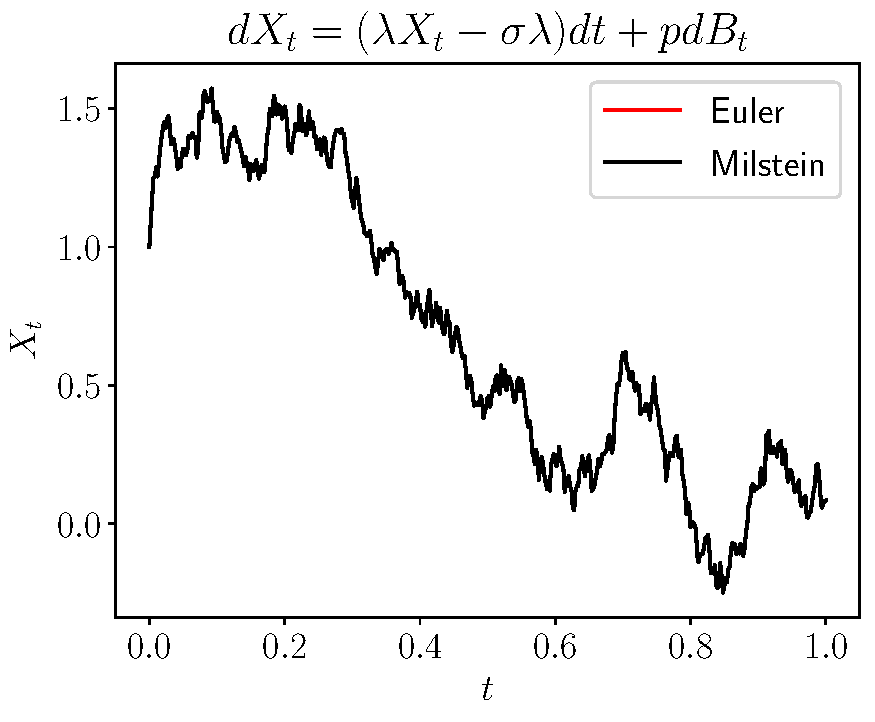
\includegraphics[scale=0.7]{files/result_punto2.pdf}
    \caption{Simulación de la EDE.}
\end{figure}
\newpage


\item Pregunta 4. c)
\begin{minted}{python}
# Run
t, x = sp.symbols('t x')
def F(t, x):
    return sp.sec(t) - sp.tan(t) * x
def G(t, x):
    return sp.sqrt(2 * sp.sec(t)) * x
x0 = 1
t0 = 0
N = 1
T = 1
delta_t = 1 / 500
f = F(t, x)
g = G(t, x)
ts, B = mbeus(delta_t, T)
xs_milstein = milstein(f, g, B, x0, t0, delta_t, T, N)
xs_euler = euler_maruyama(f, g, B, x0, t0, delta_t, T, N)
plt.plot(ts, np.transpose(xs_euler), 'r', label='Euler')
plt.plot(ts, np.transpose(xs_milstein), 'k', label='Milstein')
plt.title("$dX_t=(\mathrm{sec}(t)-\mathrm{tan}(t)X_t)dt + X_t\sqrt{2\mathrm{sec}(t)}dB_t$")
plt.xlabel("$t$")
plt.ylabel("$X_t$")
plt.legend()
plt.savefig("result.pdf", bbox_inches='tight')
plt.show()
\end{minted}

\begin{figure}[H]
    \centering
    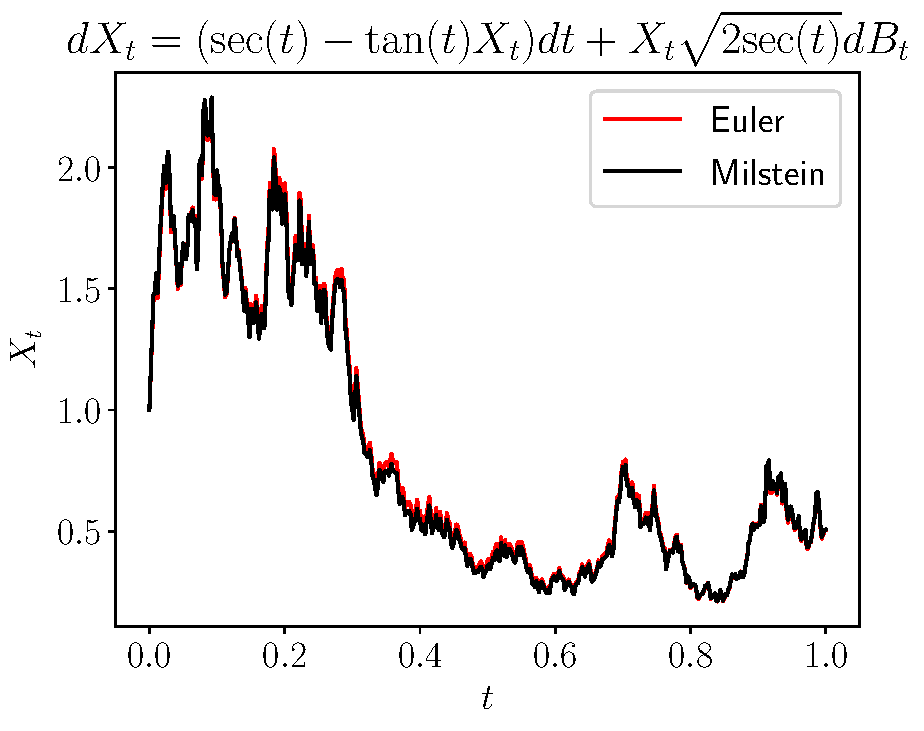
\includegraphics[scale=0.8]{files/result_punto4.pdf}
    \caption{Simulación de la EDE.}
\end{figure}
\end{enumerate}

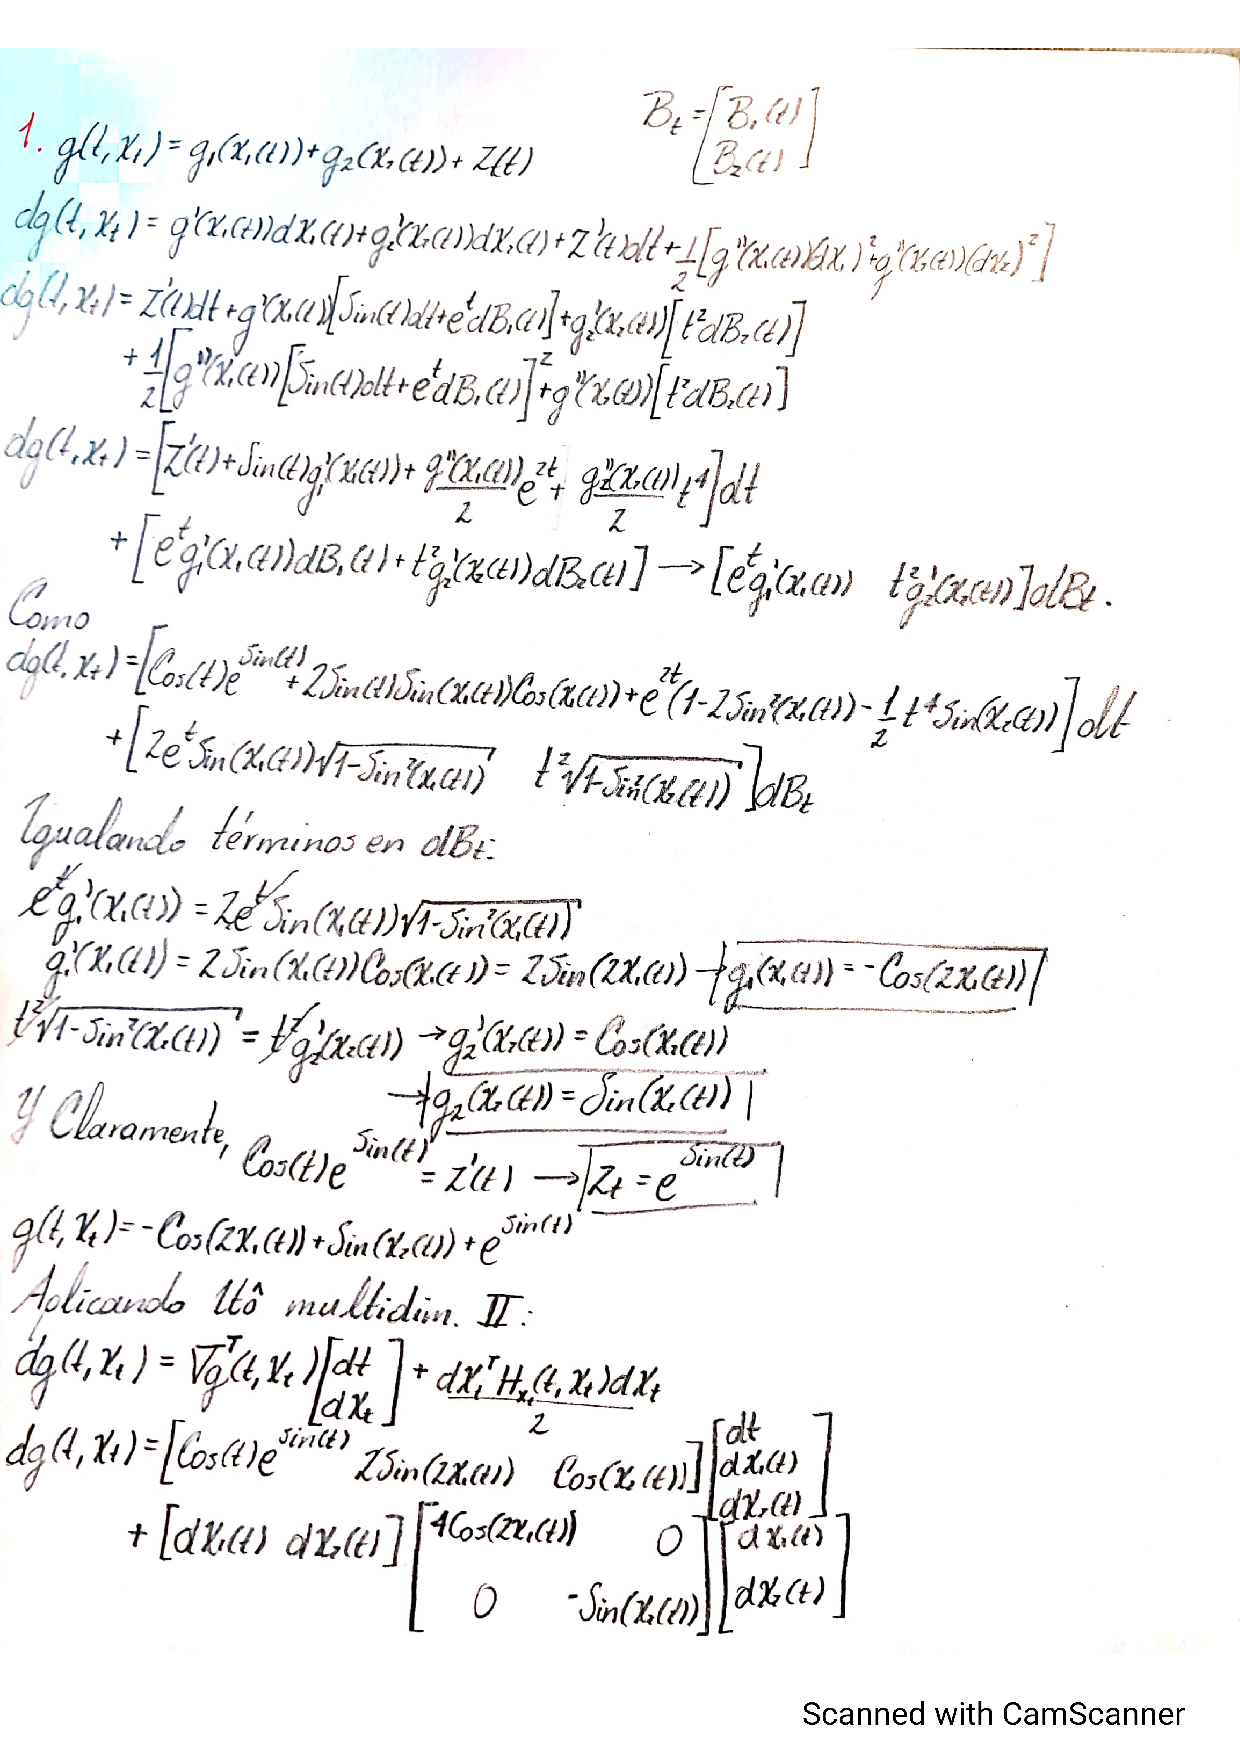
\includepdf[page=-]{files/parcial2_daples.pdf}
\end{document}
